\documentclass[minion]{homework651}

\usepackage[all,cmtip]{xy}
\usepackage{tikz}

\doclabel{Math F651: Homework 7}
\docdate{Due: March 4, 2015}
\docauthor{Kirk Hogenson}

\newcommand{\nextprob}{\newpage}
\newcommand{\RR}{\mathbb{R}}
\newcommand{\PP}{\mathbb{P}}
\newcommand{\ra}{\rightarrow}
\newcommand{\calB}{\mathcal{B}}
\newcommand{\NN}{\mathbb{N}}

\begin{document}
\begin{aproblems}
\hproblem Problem 3-14

Show that real projective space $\mathbb{P}^n$ is an $n$-manifold.
[Hint: consider the subsets $U_i \subseteq \mathbb{R}^{n+1}$ where $x_i= 1$.]

\solution
Let $V_i\subseteq \RR^{n+1}$ be $V_i=\{x\in\RR^{n+1}:x_i= 1\}$.

\textbf{Lemma:} \textit{The set $V_i$ is homeomorphic to $\RR^n$}\\
Define $i:V_i\ra\RR^n$ by $i(x_1,...,x_{n+1})=(x_1,...,\hat{x_i},...,x_{n+1})$,
where $x_i$ is omitted, and $x_i=1$ because $x\in V_i$.
Clearly $i$ is bijective and continuous, since each coordinate function is continuous.

Also, $i^{-1}$ is the map
$i^{-1}:(x_1,...,x_n)=(x_1,...,1,...,x_{n+1})$, where there is a 1
inserted
in slot $i$.  Each component function is continuous so it is
continuous and hence $i$ is a homeomorphism.\hfill$\Box$

We will denote the quotient map from $\RR^{n+1}$ to $\PP^n$ by $q$.

Let $U_i\subseteq \RR^{n+1}$ be $U_i=\{x\in\RR^{n+1}:x_i\ne 0\}$.\\

Define $\phi_i:U_i\ra V_i$ be the map
$\phi_i(x)=\frac{1}{x_i}(x_1,...,x_{n+1})$.

Then $\phi_i$ is constant on the fibers of $\PP^n$, because if
$x\sim y$ then $x_k=\lambda y_k$ for $1\le k \le n+1$, and:
$$ \phi_i(x)=\frac{1}{x_i}(x_1,...,x_{n+1})=
\frac{1}{\lambda y_i}(\lambda y_1,...,\lambda y_{n+1}) =
\frac{1}{y_i}(y_1,...,y_{n+1})=\phi_i(y). $$
Also observe that $\phi_i$ is continuous, in class we discussed that the map
``scalar multiplication'' is continuous.

So, in the diagram

\centerline{
\xymatrix{
U_i \ar[d]_{q} \ar[dr]^{\phi_i} &  \\
\PP^n \ar[r]_{\tilde\phi_i} & V_i  }}

the function $\tilde\phi_i$ exists, and furthermore it is continuous
since $\phi_i$ is continuous and $q$ is a quotient map.

Next consider this diagram

\centerline{
\xymatrix{
V_i \ar@{^{(}->}[r]^{i} \ar[dr]_{\tilde\psi_i} & \RR^n \ar[d]^{q}  \\
 & \PP^n  }}

The topological embedding from $V_i$ to $\RR^n$ is continuous from the
Lemma, and $q$ is a quotient map, hence $\tilde\psi_i$ is continuous.

Note that $\phi_i(x)=x$ if $x\in V_i$, and that $i(x)=x$ is the identity
map when $x\in V_i$.
Then $\tilde\phi_i^{-1}=\psi_i$, because
\begin{align*}
x\in V_i:\quad \tilde\phi_i(\tilde\psi_i(x)) &= \tilde\phi_i(q(i(x)))=\phi_i(i(x))=\phi_i(x)=x.\\
x\in\PP^n:\quad \tilde\psi_i(\tilde\phi_i(x)) &= q(i(\tilde\phi_i(x)))=q(\tilde\phi_i(x))=\phi_i(x)=x.
\end{align*}

Thus $\tilde\phi_i$ is a bijection from $\PP^n$ to $V_i$ and hence a homeomorphism.
In the Lemma we showed that $V_i$ is homeomorphic to $\RR^n$, so
$\PP^n$ is homeomorphic to $\RR^n$

The functions $\tilde\phi_i$ define charts on $\PP^n$ to $V_i$.  Observe that
every $x\in\PP^n$ is in the domain of at least one chart.  Hence $\PP^n$
is locally Euclidean.

$\PP^n$ is then second countable because $U_i$ is second countable.  Further,
$\PP^n$ is Hausdorff hence $\PP^n$ is an $n$ dimensional manifold.

\nextprob
\hproblem Problem 3-16

Let $X$ be the subset
$(\mathbb{R}\times\{0\})\cup(\mathbb{R}\times\{1\})\subseteq \mathbb{R}^2$.
Define an equivalence relation on $X$ by declaring $(x,0)\sim (x,1)$ if $x\neq 0$.
Show that the quotient space $X/\sim$ is locally Euclidean and second countable,
but not Hausdorff. (This space is called the line with two origins.)

Your solution should not be longer than a page.
Extra credit for the shortest correct solution.

\solution
Denote the quotient map by $q$ and
define the sets $X_0=X\setminus\{(0,1)\}$ and $X_1=X\setminus\{(0,0)\}$,
and the maps
\begin{align*}
\phi_0:X_0\ra\RR \text{ by } \phi_0(x,a) &= x  \\
\phi_1:X_1\ra\RR \text{ by } \phi_1(x,a) &= x.
\end{align*}
Each of $\phi_i$ is a projection and hence continuous.  The sets $X_0$
and $X_1$ are both open in $X$ as removing a single point results in
an open set.

Claim: $\phi_i$ is constant on the fibers of $q$. To see this,
let $q(x,a)=q(y,b)$, where $(x,a)$ and $(y,b)\in X_i$.
Then, we must have $x=y$, and hence $\phi_i(x)=\phi_i(y)$.
Thus, in the diagram

\centerline{
\xymatrix{
X_i \ar[d]_{q} \ar[dr]^{\phi_i} &  \\
X/\sim \ar[r]_{\tilde\phi_i} & \RR  }}

the map $\tilde\phi_i$ exists, and it is continuous.  In fact we can write
$\tilde\phi_i([x])=x$, and evidently $\tilde\phi_i$ is bijective.

Now consider the diagram

\centerline{
\xymatrix{
\RR \ar[r]^{f_i} \ar[dr]_{\tilde\psi_i} & X_i \ar[d]^{q}  \\
 & X/\sim  }}

Where the map $f_i:\RR\ra X_i$ is $f_i(x)=(x,i)$.  Note that $(x,i)\in X_i$,
and that $f_i$ is continuous because each component is.  Then by
the characteristic property, $\tilde\psi_i$ is continuous.
Moreover,
$\tilde\psi_i=\tilde\phi_i^{-1}$ because
\begin{align*}
\tilde\phi_i(\tilde\psi_i(x)) &= \tilde\phi_i(q(f_i(x))) =
                                 \phi_i(f_i(x)) = \phi_i(x,i) = x\\
\tilde\psi_i(\tilde\phi_i([x])) &= q(f_i(\tilde\phi_i([x]))) =
                                 q(f_i(x)) = q(x,i) = [x].
\end{align*}
Therefore $\tilde\phi_i$ is a homeomorphism.  Hence the pair $\tilde\phi_i$
are two charts on $X/\sim$ and therefore $X/\sim$ is locally
Euclidean.
Then because $X$ is second countable, $X/\sim$ is second countable.

Finally, $X/\sim$ is not Hausdorff.  To see this,
let $U_i=(a_i,b_i)\times\{i\}$ be basic open neighborhoods of
$(0,i)\in X$, for $i=0,1$.  Take any $(x,0)\in U_0$, and WLOG suppose $x>0$,
so $0<x<b_0$.  If $(x,1)\in U_1$ we are done, so suppose $(x,1)\not\in U_1$.
Then $0<b_1<x$, and choose $c$ such that $0<c<b_1$.
But then $0<c<b_0$, so $(c,0)\in U_0$ and $(c,1)\in U_1$, so
$q(U_0)\cap q(U_1)\ne\emptyset$.

\nextprob
\hproblem Exercise 4.4

Prove that a topological space $X$ is disconnected if and only if there exists a
nonconstant continuous function from $X$ to the discrete space $\{0,1\}$.

\solution
($\implies$):\\
Suppose $X$ is disconnected.  Then there exist disjoint open sets $U,V$ in $X$ where
$U$ and $V$ are nonempty, are not $X$, and with $U\cup V=X$.

Define $f:X\ra \{0,1\}$ by $f(U)=0$ and $f(V)=1$.  Since $U$ and $V$ are both
nonempty, $f$ is not constant.

There are only 4 open sets in $\{0,1\}$, and the preimage of all of them is
open:
$$ f^{-1}(\{0\})=U,\quad f^{-1}(\{1\})=V,\quad f^{-1}(\{0,1\})=X,\quad f^{-1}(\emptyset)=\emptyset. $$
So $f$ is continuous.

($\impliedby$):\\
The contrapositive of the reverse implication can be interpreted as:
If $X$ is connected, then any continuous function from $X$ to $\{0,1\}$ must
be constant.  But this is precisely Proposition 4.2 in the text.

\nextprob
\hproblem Problem 4-4

Show that the following topological spaces are not manifolds:

\begin{subproblems}
\item the union of the $x$-axis and the $y$-axis in $\mathbb{R}^2$
\item the conical surface $C\subseteq \mathbb{R}^3$ defined by
\begin{equation*}
C=\{(x,y,z):z^2=x^2+y^2\}
\end{equation*}
\end{subproblems}

\subsol

\subsol

\nextprob
\hproblem Problem 4-5

Let $M=\mathbb{S}^1\times\mathbb{R}$, and let $A=\mathbb{S}^1\times\{0\}$.
Show that the space $M/A$ obtained by collapsing $A$ to a point is homeomorphic
to the space $C$ of Problem 4-4(b), and thus is Hausdorff and second countable
but not locally Euclidean.

\solution
In this problem we will work in cylindrical coordinates.  Then a point
$(r,\theta,z)\in\RR^3$, where $r>0$, $\theta\in[0,2\pi)$,
and $z\in\RR$, is in $M$ if $r=1$, and it is in $C$ if $r=|z|$.

Define a function $f:M\ra C$ by $f(1,\theta,z)=(|z|,\theta,z)$. Then
from the above the codomain of $M$ is $C$.  Also note that $f$ is
clearly surjective, as any $(|z|,\theta,z)\in C$ is evidently mapped to
by $(1,\theta,z)\in M$.

Now consider the diagram

\centerline{
\xymatrix{
M \ar[d]_{q} \ar[dr]^{f} &  \\
M/A \ar@{.>}[r]_{\tilde f} & C  }}

We've used $q$ to denote the quotient map from $M$ to $M/A$. The diagram will
show that $\tilde f$ exists and is continuous, provided that we can show
$f$ is constant on the fibers of $q$, and that $f$ is continuous.

The function $f$ is continuous if its component functions are, and each
component function here, $f_1(x,y,z)=|z|, f_2(x,y,z)=y$, and $f_3(x,y,z)=z$
is continuous.

Suppose that $q(1,\theta_1,z_1)=q(1,\theta_2,z_2)$.
This means either (i)
$\theta_1=\theta_2$ and $z_1=z_2$, or (ii) $z_1=z_2=0$.  In case (i), then clearly
$f(1,\theta_1,z_1)=f(1,\theta_2,z_2)$.  In case (ii), we have
$f(1,\theta_1,0) = (0,\theta_1,0)$ and $f(1,\theta_2,0)=(0,\theta_2,0)$, which is
the same point in cylindrical coordinates, so $f$ is constant on the fibers of $q$.

Therefore $f$ descends to the quotient and $\tilde f$ exists and is continuous.
Further, since $f$ is surjective, $\tilde f$ is bijective.

Next, consider the map $p:C\ra M$ defined by $p(r,\theta,z)=(1,\theta,z)$.
Observe that $p$ 
is continuous, since each component is continuous.

Then in this diagram:

\centerline{
\xymatrix{
C \ar[r]^{p} \ar[dr]_{g} & M \ar[d]^{q}  \\
 & M/A  }}

We have that the function $g$ is continuous, since $p$ is and $q$ is a quotient
map and hence continuous.

Also, we can now write:
$$ (\tilde f\circ g)(r,\theta,z)=\tilde f(q(p(r,\theta,z)))=f(p(r,\theta,z)=
   f(1,\theta,z)=(|z|,\theta,z). $$
Since the original point $(r,\theta,z)$ was in $C$, it satisfied $r=|z|$, hence
$\tilde f=g^{-1}$.  Since $\tilde f$ is bijective, we also have $\tilde f^{-1}=g$,
which means that $\tilde f$ is continuous.

Therefore $\tilde f$ is a homeomorphism, and $M/A$ is homeomorphic to $C$.
Thus, because $C$ is Hausdorff and second countable but not locally Euclidean,
$M/A$ is as well.

\nextprob
\hproblem Let $X$ be a topological space with components $\{C_\alpha\}$.
Show that $X$ has the disjoint union topology $\coprod C_\alpha$ if and only if
each $C_\alpha$ is open.

\solution
Suppose $X$ has the disjoint union topology defined by $\coprod C_\alpha$,
and choose any $x\in C_\alpha$ for some $\alpha$.
Let $U$ be an open set in $X$ with $x\in U$.  Then
by the disjoint union topology, $U\cap C_\alpha$ is open in $C_\alpha$,
hence $C_\alpha$ is open.

Suppose each $C_\alpha$ is open.  Observe that for any $U\subseteq X$:
$$U=X\cap U=\left(\bigcup_{\alpha\in I} C_\alpha\right)\cap U=
  \bigcup_{\alpha\in I} (C_\alpha \cap U).$$
If $U$ is open in $X$, each $C_\alpha \cap U$ is also open,
hence $U$ is an open set in the disjoint union topology $\coprod C_\alpha$.
Conversely, if each $C_\alpha\cap U$ is open in $C_\alpha$, then $U$ is
open in $X$.  Hence, the open sets in the topology on $X$ and the
disjoint union topology are the same.

\nextprob
\hproblem Problem 4-9 (Just the manifold part)

Show that every $n$-manifold is homeomorphic to a disjoint union of countably
many connected $n$-manifolds.

\solution
Let $M$ be an $n$-manifold.  Let $\{C_\alpha\}_{\alpha\in I}$
be the connected components of
$M$.  Since $M$ is a disjoint union of $\{C_\alpha\}$, each $C_\alpha$ is
open by the previous excercise.  Any open subset of an $n$-manifold is itself
an $n$-manifold, hence each $C_\alpha$ is an $n$-manifold.

Manifolds are second countable, hence $M$ has a countable basis.  Let $\calB$ be
a countable basis for $M$.  Choose any $x_\alpha$ in each $C_\alpha$.  Then
there is a $B_\alpha\in\calB$ with $x_\alpha\in B_\alpha\subseteq C_\alpha$,
for each $\alpha\in I$.

Define the function $f:I\ra I$ by $f(\alpha)=\beta$ where 
$\beta$ is the $\beta$ for which $B_\beta\subseteq C_\alpha$.  Clearly
$f$ is surjective, as there is a $B_\beta$ for each $C_\alpha$.

For any $\alpha_1,\alpha_2 \in I$, where $\alpha_1\ne\alpha_2$,
we have $C_{\alpha_1} \cap C_{\alpha_2} = \emptyset$ hence
$B_{f(\alpha_1)} \cap B_{f(\alpha_2)} = \emptyset$ too,
and so $B_{f(\alpha_1)} \ne B_{f(\alpha_2)}$.
Thus $f$ is injective, and hence we have a bijection between a
subset of $\calB$ and 
$\{C_\alpha\}$.  Since $\calB$ is countable, $\{C_\alpha\}$
must be as well.

\nextprob
\hproblem Problem 4-13

Define subsets of the plane by
\begin{align*}
T_0 &= \{(x,y) : x=0 \text{ and } y\in[-1,1]\}; \\
T_+ &= \{(x,y) : x\in(0,2\pi] \text{ and } y=\sin(1/x)\}.
\end{align*}

Let $T = T_0\cup T_+$.
The space $T$ is called the \textbf{\emph{topologist's sine curve}}.

\begin{subproblems}
\item Show that $T$ is connected but not path-connected or locally connected.
\item Determine the components and the path components of $T$.
\end{subproblems}

\begin{center}
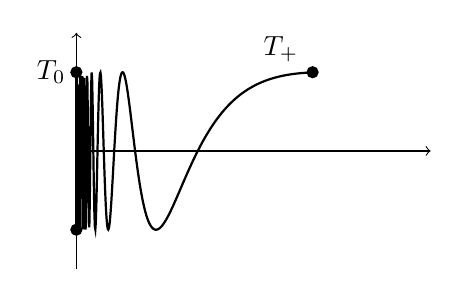
\begin{tikzpicture}[x=5cm]
    %\draw[xstep=.2,ystep=.5,lightgray,ultra thin] (-0.1,-1.5) grid (1.1,1.5);
    \draw[->] (0,0) -- (.9,0);
    \draw[->] (0,-1.5) -- (0,1.5);
    \draw[very thick] (0,-1) -- (0,1) node[left] {$T_0$};
    \filldraw (0,-1) circle (2pt);
    \filldraw (0,1) circle (2pt);
    \filldraw (.6,1) circle (2pt);
  \draw[thick,domain=0.01:.6,samples=500] plot (\x-.01, {sin((1/\x)r)}) node[above left] {$T_+$};
\end{tikzpicture}
\end{center}

\textbf{Lemma:} \textit{$\overline{T_+}=T=T_0 \cup T_+$}\\
%Let $(x,y)\in T_0\cup T_+$.  If $(x,y)\in T_+$ then it is in $\overline{T_+}$.
%If $(x,y)\in T_0$, then $x=0$ and $y\in[-1,1]$.  Let $B_r(0,y)$ be an open
%ball centered at $(0,y)$, and pick $(x, y)$ in $B_r(0,y)$, with $x>0$.
%Then choose
%an $x'$ small enough so that $1/x' > 1/x$, and $y=\sin(1/x')$. This can
%be done by selecting any $z$ for which $\sin(z)=y$, and choosing $n\in\NN$
%so that $z+2n\pi>1/x$, and taking $x'=1/(z+2n\pi)$.
%Then
%$x'<x$ and $(x',y)\in T_+$, and $(x',y)\in B_r(x,y)$.  Thus
%$B_r(x,y)\cap T_+\ne\emptyset$, showing that $T_0\cup T_+\subseteq \overline{T_+}$.
Take any $P=(x,y)\in\RR^2$.  If $x<0$, then $B_{-x}(x,y)\cap T=\emptyset$, so
$P\not\in\overline{T_+}$.  If $x>0$ and $y=\sin(1/x)$, then $P\in T_+$.
If $x>0$ and $y\ne \sin(1/x)$, let $d$ be the distance from $(x,y)$ to the
curve $y=\sin(1/x)$, and then $B_d(x,y)\cap T=\emptyset$.
If $|y|>1$, then $B_r(x,y)\cap T=\emptyset$ if we take
$r=(|y|-1)/2$.  The only points in $\RR^2$ left are in $T_0$.  We've just
shown that every point in $\RR^2$ is not in $\overline{T_+}$, or it is
in $T_0\cup T_+$, hence $\overline{T_+}=T$.

\subsol
Observe that $T_+$ is connected, since it is the image of a continuous
function of a connected set, $(0,2\pi]$.  Hence $\overline{T_+}$ is
connected. From the Lemma, $\overline{T_+}=T$ so $T$ is connected.

Suppose $T$ is path connected. Let $a=(0,0)$ and $b=(2/\pi,1)$, and
choose a path function $\gamma:[0,1]\ra T$,
with $\gamma(0)=a$ and $\gamma(1)=b$.  Let $B_r(a)$ be a ball of
radius $r=1/2$ around $a$.
Since $\gamma$ is continuous, $\gamma(t)$ must eventually be in $B_r(a)$,
that is, for some $t_0>0$ we will have $\gamma(t)\in B_r(a)$ if $t<t_0$.
Choose $t_1<t_0$, and let $(x,y)=\gamma(t_1)$.  Then for any $x'<x$, we
must have $(x',\sin(1/x'))\in B_r(a)$.  But, there
are infinitely many points less than $x$ for which $\sin(1/x)=1$.  Hence
$T$ is not path connected.

Further, $T$ is not locally connected, 

\subsol
Since $T$ is connected, it has only one connected component, $T$ itself.

$T_0$ is path connected, it is a closed interval in $\RR$ embedded in $\RR^2$.
$T_+$ is path connected, it is the image under a continuous function of a
path connected set.  But $T$ is not path connected, hence it has 2 path
components, $T_0$ and $T_+$.

\end{aproblems}
\end{document}

